% Options for packages loaded elsewhere
\PassOptionsToPackage{unicode}{hyperref}
\PassOptionsToPackage{hyphens}{url}
%
\documentclass[
]{article}
\usepackage{amsmath,amssymb}
\usepackage{lmodern}
\usepackage{iftex}
\ifPDFTeX
  \usepackage[T1]{fontenc}
  \usepackage[utf8]{inputenc}
  \usepackage{textcomp} % provide euro and other symbols
\else % if luatex or xetex
  \usepackage{unicode-math}
  \defaultfontfeatures{Scale=MatchLowercase}
  \defaultfontfeatures[\rmfamily]{Ligatures=TeX,Scale=1}
\fi
% Use upquote if available, for straight quotes in verbatim environments
\IfFileExists{upquote.sty}{\usepackage{upquote}}{}
\IfFileExists{microtype.sty}{% use microtype if available
  \usepackage[]{microtype}
  \UseMicrotypeSet[protrusion]{basicmath} % disable protrusion for tt fonts
}{}
\makeatletter
\@ifundefined{KOMAClassName}{% if non-KOMA class
  \IfFileExists{parskip.sty}{%
    \usepackage{parskip}
  }{% else
    \setlength{\parindent}{0pt}
    \setlength{\parskip}{6pt plus 2pt minus 1pt}}
}{% if KOMA class
  \KOMAoptions{parskip=half}}
\makeatother
\usepackage{xcolor}
\usepackage[margin=1in]{geometry}
\usepackage{color}
\usepackage{fancyvrb}
\newcommand{\VerbBar}{|}
\newcommand{\VERB}{\Verb[commandchars=\\\{\}]}
\DefineVerbatimEnvironment{Highlighting}{Verbatim}{commandchars=\\\{\}}
% Add ',fontsize=\small' for more characters per line
\usepackage{framed}
\definecolor{shadecolor}{RGB}{248,248,248}
\newenvironment{Shaded}{\begin{snugshade}}{\end{snugshade}}
\newcommand{\AlertTok}[1]{\textcolor[rgb]{0.94,0.16,0.16}{#1}}
\newcommand{\AnnotationTok}[1]{\textcolor[rgb]{0.56,0.35,0.01}{\textbf{\textit{#1}}}}
\newcommand{\AttributeTok}[1]{\textcolor[rgb]{0.77,0.63,0.00}{#1}}
\newcommand{\BaseNTok}[1]{\textcolor[rgb]{0.00,0.00,0.81}{#1}}
\newcommand{\BuiltInTok}[1]{#1}
\newcommand{\CharTok}[1]{\textcolor[rgb]{0.31,0.60,0.02}{#1}}
\newcommand{\CommentTok}[1]{\textcolor[rgb]{0.56,0.35,0.01}{\textit{#1}}}
\newcommand{\CommentVarTok}[1]{\textcolor[rgb]{0.56,0.35,0.01}{\textbf{\textit{#1}}}}
\newcommand{\ConstantTok}[1]{\textcolor[rgb]{0.00,0.00,0.00}{#1}}
\newcommand{\ControlFlowTok}[1]{\textcolor[rgb]{0.13,0.29,0.53}{\textbf{#1}}}
\newcommand{\DataTypeTok}[1]{\textcolor[rgb]{0.13,0.29,0.53}{#1}}
\newcommand{\DecValTok}[1]{\textcolor[rgb]{0.00,0.00,0.81}{#1}}
\newcommand{\DocumentationTok}[1]{\textcolor[rgb]{0.56,0.35,0.01}{\textbf{\textit{#1}}}}
\newcommand{\ErrorTok}[1]{\textcolor[rgb]{0.64,0.00,0.00}{\textbf{#1}}}
\newcommand{\ExtensionTok}[1]{#1}
\newcommand{\FloatTok}[1]{\textcolor[rgb]{0.00,0.00,0.81}{#1}}
\newcommand{\FunctionTok}[1]{\textcolor[rgb]{0.00,0.00,0.00}{#1}}
\newcommand{\ImportTok}[1]{#1}
\newcommand{\InformationTok}[1]{\textcolor[rgb]{0.56,0.35,0.01}{\textbf{\textit{#1}}}}
\newcommand{\KeywordTok}[1]{\textcolor[rgb]{0.13,0.29,0.53}{\textbf{#1}}}
\newcommand{\NormalTok}[1]{#1}
\newcommand{\OperatorTok}[1]{\textcolor[rgb]{0.81,0.36,0.00}{\textbf{#1}}}
\newcommand{\OtherTok}[1]{\textcolor[rgb]{0.56,0.35,0.01}{#1}}
\newcommand{\PreprocessorTok}[1]{\textcolor[rgb]{0.56,0.35,0.01}{\textit{#1}}}
\newcommand{\RegionMarkerTok}[1]{#1}
\newcommand{\SpecialCharTok}[1]{\textcolor[rgb]{0.00,0.00,0.00}{#1}}
\newcommand{\SpecialStringTok}[1]{\textcolor[rgb]{0.31,0.60,0.02}{#1}}
\newcommand{\StringTok}[1]{\textcolor[rgb]{0.31,0.60,0.02}{#1}}
\newcommand{\VariableTok}[1]{\textcolor[rgb]{0.00,0.00,0.00}{#1}}
\newcommand{\VerbatimStringTok}[1]{\textcolor[rgb]{0.31,0.60,0.02}{#1}}
\newcommand{\WarningTok}[1]{\textcolor[rgb]{0.56,0.35,0.01}{\textbf{\textit{#1}}}}
\usepackage{graphicx}
\makeatletter
\def\maxwidth{\ifdim\Gin@nat@width>\linewidth\linewidth\else\Gin@nat@width\fi}
\def\maxheight{\ifdim\Gin@nat@height>\textheight\textheight\else\Gin@nat@height\fi}
\makeatother
% Scale images if necessary, so that they will not overflow the page
% margins by default, and it is still possible to overwrite the defaults
% using explicit options in \includegraphics[width, height, ...]{}
\setkeys{Gin}{width=\maxwidth,height=\maxheight,keepaspectratio}
% Set default figure placement to htbp
\makeatletter
\def\fps@figure{htbp}
\makeatother
\setlength{\emergencystretch}{3em} % prevent overfull lines
\providecommand{\tightlist}{%
  \setlength{\itemsep}{0pt}\setlength{\parskip}{0pt}}
\setcounter{secnumdepth}{-\maxdimen} % remove section numbering
\ifLuaTeX
  \usepackage{selnolig}  % disable illegal ligatures
\fi
\IfFileExists{bookmark.sty}{\usepackage{bookmark}}{\usepackage{hyperref}}
\IfFileExists{xurl.sty}{\usepackage{xurl}}{} % add URL line breaks if available
\urlstyle{same} % disable monospaced font for URLs
\hypersetup{
  hidelinks,
  pdfcreator={LaTeX via pandoc}}

\author{}
\date{\vspace{-2.5em}}

\begin{document}

This practical is based on exploratory data analysis and prediction of a
dataset derived from a municipal database of healthcare administrative
data. This dataset is derived from Vitoria, the capital city of Espírito
Santo, Brazil (population 1.8 million) and was freely shared under a
creative commons license.

\textbf{Generate an rmarkdown report that contains all the necessary
code to document and perform: EDA, prediction of no-shows using XGBoost,
and an analysis of variable/feature importance using this data set.
Ensure your report includes answers to any questions marked in bold.
Please submit your report via brightspace as a link to a git repository
containing the rmarkdown and compiled/knitted html version of the
notebook.}

\hypertarget{introduction}{%
\subsection{Introduction}\label{introduction}}

The Brazilian public health system, known as SUS for Unified Health
System in its acronym in Portuguese, is one of the largest health system
in the world, representing government investment of more than 9\% of
GDP. However, its operation is not homogeneous and there are distinct
perceptions of quality from citizens in different regions of the
country. Non-attendance of medical appointments contributes a
significant additional burden on limited medical resources. This
analysis will try and investigate possible factors behind non-attendance
using an administrative database of appointment data from Vitoria,
Espírito Santo, Brazil.

The data required is available via the
\href{https://github.com/maguire-lab/health_data_science_research/tree/master/static_files/practicals/lab1_data}{course
website}.

\hypertarget{understanding-the-data}{%
\subsubsection{Understanding the data}\label{understanding-the-data}}

\textbf{1} Use the data dictionary describe each of the
variables/features in the CSV in your report.

PatientID is unique identifier for each patient therefore they cannot be
directly identified from their name etc. for ethical purposes.

AppointmentID is a unique identifier to each appointment for
confidentiality, as described above

Gender indicates the patient's gender, which is Male or Female

ScheduledDate is the date when the appointment was scheduled

AppointmentDate is the date of the actual appointment when the
individual comes in

Age is the Patient's age (in years)

Neighbourhood is the District of Vitória where the appointment takes
place (Southeastern coast of Brazil)

SocialWelfare is if the Patient is a recipient of Bolsa Família welfare
payments (payments from the social welfare of the government of Brazil)

Hypertension is if the Patient was previously diagnoised with
hypertension before appointment (1 yes/ 0 no)

Diabetes is if the Patient was previously diagnosed with diabetes before
appointment (1 yes/ 0 no)

AlcoholUseDisorder is if the Patient was previously diagnosed with
alcohol use disorder before appointment (1 yes/ 0 no)

Disability is if the Patient was previously diagnosed with a disability
before the appointment (severity rated 0-4)

SMSReceived is at least 1 reminder text sent before appointment (1 yes/
0 no)

NoShow is if the Patient did not show up scheduled appointment (Yes/No)

\textbf{2} Can you think of 3 hypotheses for why someone may be more
likely to miss a medical appointment?

\begin{enumerate}
\def\labelenumi{\arabic{enumi}.}
\item
  Low socioeconomic status (may not have transportation or ability to
  get there)
\item
  Older Age (may forget about appointment or may not be able to
  physically get there without assistance)
\item
  Mental health and addiction issues (may not want to go there
  (embarassment/stigma surrounding addictions) or may not have
  resourses/transportation to get there)
\end{enumerate}

\textbf{3} Can you provide 3 examples of important contextual
information that is missing in this data dictionary and dataset that
could impact your analyses e.g., what type of medical appointment does
each \texttt{AppointmentID} refer to?\\
1. Distance from place of residence to appointment site (could be a
major factor to predicting no shows, as the more time individuals have
to spend to get to their appointment, maybe the less likely they are to
attend it)

\begin{enumerate}
\def\labelenumi{\arabic{enumi}.}
\setcounter{enumi}{1}
\item
  Number of admissions to hospital (this would be helpful to know if
  patients were admitted to the hospital following an appointment and
  could be the reason for many appointments if they have a disease or
  chronic condition)
\item
  Type of disability (this could be helpful for predicting no shows and
  could be a proxy to determine if individuals need assistance getting
  to their appointments)
\end{enumerate}

\hypertarget{data-parsing-and-cleaning}{%
\subsection{Data Parsing and Cleaning}\label{data-parsing-and-cleaning}}

\textbf{4} Modify the following to make it reproducible i.e., downloads
the data file directly from version control

\begin{Shaded}
\begin{Highlighting}[]
\NormalTok{raw.data }\OtherTok{\textless{}{-}} \FunctionTok{read\_csv}\NormalTok{(}\StringTok{\textquotesingle{}2016\_05v2\_VitoriaAppointmentData.csv\textquotesingle{}}\NormalTok{, }\AttributeTok{col\_types=}\StringTok{\textquotesingle{}fffTTifllllflf\textquotesingle{}}\NormalTok{)}
\NormalTok{raw.data }\OtherTok{\textless{}{-}}\NormalTok{ readr}\SpecialCharTok{::}\FunctionTok{read\_csv}\NormalTok{(}\StringTok{\textquotesingle{}https://raw.githubusercontent.com/allyseamone/AppliedHealthDataScience/main/2016\_05v2\_VitoriaAppointmentData.csv\textquotesingle{}}\NormalTok{, }\AttributeTok{col\_types=}\StringTok{\textquotesingle{}fffTTifllllflf\textquotesingle{}}\NormalTok{)}
\end{Highlighting}
\end{Shaded}

\begin{verbatim}
## `curl` package not installed, falling back to using `url()`
\end{verbatim}

Now we need to check data is valid: because we specified col\_types and
the data parsed without error most of our data seems to at least be
formatted as we expect i.e., ages are integers

\begin{Shaded}
\begin{Highlighting}[]
\NormalTok{raw.data }\SpecialCharTok{\%\textgreater{}\%} \FunctionTok{filter}\NormalTok{(Age }\SpecialCharTok{\textgreater{}} \DecValTok{110}\NormalTok{)}
\end{Highlighting}
\end{Shaded}

\begin{verbatim}
## # A tibble: 5 x 14
##   PatientID   AppointmentID Gender ScheduledDate       AppointmentDate       Age
##   <fct>       <fct>         <fct>  <dttm>              <dttm>              <int>
## 1 3196321161~ 5700278       F      2016-05-16 09:17:44 2016-05-19 00:00:00   115
## 2 3196321161~ 5700279       F      2016-05-16 09:17:44 2016-05-19 00:00:00   115
## 3 3196321161~ 5562812       F      2016-04-08 14:29:17 2016-05-16 00:00:00   115
## 4 3196321161~ 5744037       F      2016-05-30 09:44:51 2016-05-30 00:00:00   115
## 5 7482345792~ 5717451       F      2016-05-19 07:57:56 2016-06-03 00:00:00   115
## # i 8 more variables: Neighbourhood <fct>, SocialWelfare <lgl>,
## #   Hypertension <lgl>, Diabetes <lgl>, AlcoholUseDisorder <lgl>,
## #   Disability <fct>, SMSReceived <lgl>, NoShow <fct>
\end{verbatim}

We can see there are 2 patient's older than 100 which seems suspicious
but we can't actually say if this is impossible.

\textbf{5} Are there any individuals with impossible ages? If so we can
drop this row using \texttt{filter} i.e.,
\texttt{data\ \textless{}-\ data\ \%\textgreater{}\%\ filter(CRITERIA)}

While there are two people that are 115 years old, we cannot actually
tell if this is an impossible age. One of the individuals does have
hypertension, which can be managed using medication, but it may not be
biologically plausible for an individual to live to 115 years while
having hypertension. It also says that the individual did receive a text
message reminder, in this day and age a lot of individuals do have cell
phones; an individual that is 115 years old may not have a cell phone.
This age may be an imputation error or it could be correct, but these
should be considered with caution as they are borderline biologically
implausible. These individuals will be kept in the data set but when
interpreting results, there should be considerations for these
individuals. Since there are 110 527 observations, these 2 individuals
should not skew the data or analyses.

\hypertarget{exploratory-data-analysis}{%
\subsection{Exploratory Data Analysis}\label{exploratory-data-analysis}}

First, we should get an idea if the data meets our expectations, there
are newborns in the data (\texttt{Age==0}) and we wouldn't expect any of
these to be diagnosed with Diabetes, Alcohol Use Disorder, and
Hypertension (although in theory it could be possible). We can easily
check this:

\begin{Shaded}
\begin{Highlighting}[]
\NormalTok{raw.data }\SpecialCharTok{\%\textgreater{}\%} \FunctionTok{filter}\NormalTok{(Age }\SpecialCharTok{==} \DecValTok{0}\NormalTok{) }\SpecialCharTok{\%\textgreater{}\%} \FunctionTok{select}\NormalTok{(Hypertension, Diabetes, AlcoholUseDisorder) }\SpecialCharTok{\%\textgreater{}\%} \FunctionTok{unique}\NormalTok{()}
\end{Highlighting}
\end{Shaded}

\begin{verbatim}
## # A tibble: 1 x 3
##   Hypertension Diabetes AlcoholUseDisorder
##   <lgl>        <lgl>    <lgl>             
## 1 FALSE        FALSE    FALSE
\end{verbatim}

We can also explore things like how many different neighborhoods are
there and how many appoints are from each?

\begin{Shaded}
\begin{Highlighting}[]
\FunctionTok{count}\NormalTok{(raw.data, Neighbourhood, }\AttributeTok{sort =} \ConstantTok{TRUE}\NormalTok{)}
\end{Highlighting}
\end{Shaded}

\begin{verbatim}
## # A tibble: 81 x 2
##    Neighbourhood         n
##    <fct>             <int>
##  1 JARDIM CAMBURI     7717
##  2 MARIA ORTIZ        5805
##  3 RESISTÊNCIA        4431
##  4 JARDIM DA PENHA    3877
##  5 ITARARÉ            3514
##  6 CENTRO             3334
##  7 TABUAZEIRO         3132
##  8 SANTA MARTHA       3131
##  9 JESUS DE NAZARETH  2853
## 10 BONFIM             2773
## # i 71 more rows
\end{verbatim}

\textbf{6} What is the maximum number of appointments from the same
patient?

The maximum number of appointments from the same patient
(822145925426128) is 88.They did not show up to a lot of their
appointments though.

\begin{Shaded}
\begin{Highlighting}[]
\FunctionTok{count}\NormalTok{(raw.data, PatientID, }\AttributeTok{sort =} \ConstantTok{TRUE}\NormalTok{)}
\end{Highlighting}
\end{Shaded}

\begin{verbatim}
## # A tibble: 62,299 x 2
##    PatientID           n
##    <fct>           <int>
##  1 822145925426128    88
##  2 99637671331        84
##  3 26886125921145     70
##  4 33534783483176     65
##  5 258424392677       62
##  6 871374938638855    62
##  7 6264198675331      62
##  8 75797461494159     62
##  9 66844879846766     57
## 10 872278549442       55
## # i 62,289 more rows
\end{verbatim}

Let's explore the correlation between variables:

\begin{Shaded}
\begin{Highlighting}[]
\CommentTok{\# let\textquotesingle{}s define a plotting function}
\NormalTok{corplot }\OtherTok{=} \ControlFlowTok{function}\NormalTok{(df)\{}
  
\NormalTok{  cor\_matrix\_raw }\OtherTok{\textless{}{-}} \FunctionTok{round}\NormalTok{(}\FunctionTok{cor}\NormalTok{(df),}\DecValTok{2}\NormalTok{)}
\NormalTok{  cor\_matrix }\OtherTok{\textless{}{-}} \FunctionTok{melt}\NormalTok{(cor\_matrix\_raw)}
  
  
  \CommentTok{\#Get triangle of the correlation matrix}
  \CommentTok{\#Lower Triangle}
\NormalTok{  get\_lower\_tri}\OtherTok{\textless{}{-}}\ControlFlowTok{function}\NormalTok{(cor\_matrix\_raw)\{}
\NormalTok{    cor\_matrix\_raw[}\FunctionTok{upper.tri}\NormalTok{(cor\_matrix\_raw)] }\OtherTok{\textless{}{-}} \ConstantTok{NA}
    \FunctionTok{return}\NormalTok{(cor\_matrix\_raw)}
\NormalTok{  \}}
  
  \CommentTok{\# Upper Triangle}
\NormalTok{  get\_upper\_tri }\OtherTok{\textless{}{-}} \ControlFlowTok{function}\NormalTok{(cor\_matrix\_raw)\{}
\NormalTok{    cor\_matrix\_raw[}\FunctionTok{lower.tri}\NormalTok{(cor\_matrix\_raw)]}\OtherTok{\textless{}{-}} \ConstantTok{NA}
    \FunctionTok{return}\NormalTok{(cor\_matrix\_raw)}
\NormalTok{  \}}
  
\NormalTok{  upper\_tri }\OtherTok{\textless{}{-}} \FunctionTok{get\_upper\_tri}\NormalTok{(cor\_matrix\_raw)}
  
  \CommentTok{\# Melt the correlation matrix}
\NormalTok{  cor\_matrix }\OtherTok{\textless{}{-}} \FunctionTok{melt}\NormalTok{(upper\_tri, }\AttributeTok{na.rm =} \ConstantTok{TRUE}\NormalTok{)}
  
  \CommentTok{\# Heatmap Plot}
\NormalTok{  cor\_graph }\OtherTok{\textless{}{-}} \FunctionTok{ggplot}\NormalTok{(}\AttributeTok{data =}\NormalTok{ cor\_matrix, }\FunctionTok{aes}\NormalTok{(Var2, Var1, }\AttributeTok{fill =}\NormalTok{ value))}\SpecialCharTok{+}
    \FunctionTok{geom\_tile}\NormalTok{(}\AttributeTok{color =} \StringTok{"white"}\NormalTok{)}\SpecialCharTok{+}
    \FunctionTok{scale\_fill\_gradient2}\NormalTok{(}\AttributeTok{low =} \StringTok{"darkorchid"}\NormalTok{, }\AttributeTok{high =} \StringTok{"orangered"}\NormalTok{, }\AttributeTok{mid =} \StringTok{"grey50"}\NormalTok{, }
                         \AttributeTok{midpoint =} \DecValTok{0}\NormalTok{, }\AttributeTok{limit =} \FunctionTok{c}\NormalTok{(}\SpecialCharTok{{-}}\DecValTok{1}\NormalTok{,}\DecValTok{1}\NormalTok{), }\AttributeTok{space =} \StringTok{"Lab"}\NormalTok{, }
                         \AttributeTok{name=}\StringTok{"Pearson}\SpecialCharTok{\textbackslash{}n}\StringTok{Correlation"}\NormalTok{) }\SpecialCharTok{+}
    \FunctionTok{theme\_minimal}\NormalTok{()}\SpecialCharTok{+} 
    \FunctionTok{theme}\NormalTok{(}\AttributeTok{axis.text.x =} \FunctionTok{element\_text}\NormalTok{(}\AttributeTok{angle =} \DecValTok{45}\NormalTok{, }\AttributeTok{vjust =} \DecValTok{1}\NormalTok{, }
                                     \AttributeTok{size =} \DecValTok{8}\NormalTok{, }\AttributeTok{hjust =} \DecValTok{1}\NormalTok{))}\SpecialCharTok{+}
    \FunctionTok{coord\_fixed}\NormalTok{()}\SpecialCharTok{+} \FunctionTok{geom\_text}\NormalTok{(}\FunctionTok{aes}\NormalTok{(Var2, Var1, }\AttributeTok{label =}\NormalTok{ value), }\AttributeTok{color =} \StringTok{"black"}\NormalTok{, }\AttributeTok{size =} \DecValTok{2}\NormalTok{) }\SpecialCharTok{+}
    \FunctionTok{theme}\NormalTok{(}
      \AttributeTok{axis.title.x =} \FunctionTok{element\_blank}\NormalTok{(),}
      \AttributeTok{axis.title.y =} \FunctionTok{element\_blank}\NormalTok{(),}
      \AttributeTok{panel.grid.major =} \FunctionTok{element\_blank}\NormalTok{(),}
      \AttributeTok{panel.border =} \FunctionTok{element\_blank}\NormalTok{(),}
      \AttributeTok{panel.background =} \FunctionTok{element\_blank}\NormalTok{(),}
      \AttributeTok{axis.ticks =} \FunctionTok{element\_blank}\NormalTok{())}\SpecialCharTok{+}
      \FunctionTok{ggtitle}\NormalTok{(}\StringTok{"Correlation Heatmap"}\NormalTok{)}\SpecialCharTok{+}
      \FunctionTok{theme}\NormalTok{(}\AttributeTok{plot.title =} \FunctionTok{element\_text}\NormalTok{(}\AttributeTok{hjust =} \FloatTok{0.5}\NormalTok{))}
  
\NormalTok{  cor\_graph}
\NormalTok{\}}

\NormalTok{numeric.data }\OtherTok{=} \FunctionTok{mutate\_all}\NormalTok{(raw.data, }\ControlFlowTok{function}\NormalTok{(x) }\FunctionTok{as.numeric}\NormalTok{(x))}

\CommentTok{\# Plot Correlation Heatmap}
\FunctionTok{corplot}\NormalTok{(numeric.data)}
\end{Highlighting}
\end{Shaded}

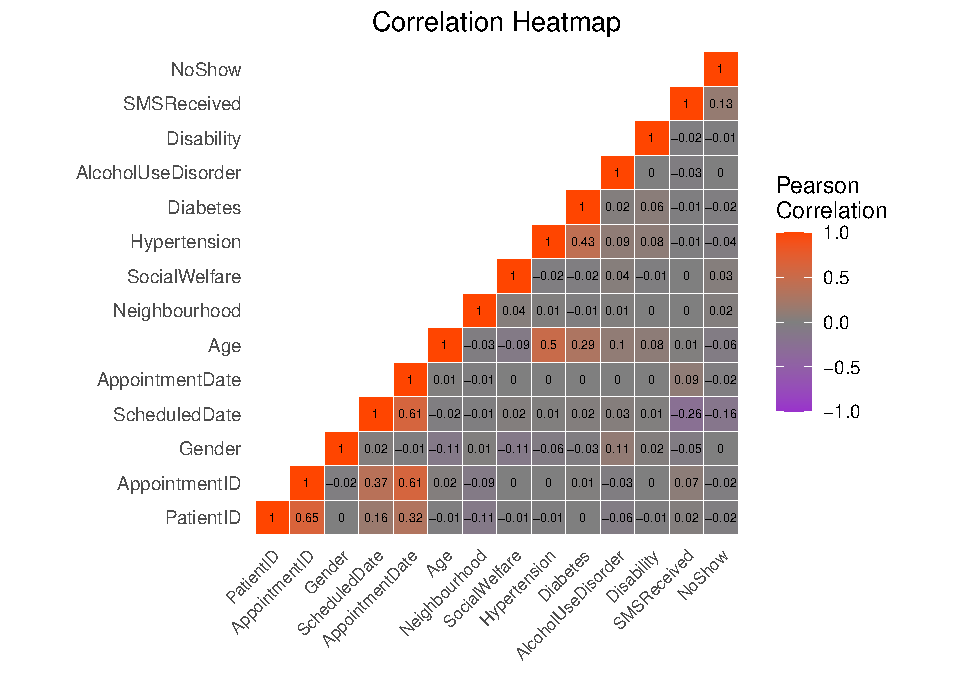
\includegraphics{lab1_medical_databases_files/figure-latex/unnamed-chunk-5-1.pdf}

Correlation heatmaps are useful for identifying linear relationships
between variables/features. In this case, we are particularly interested
in relationships between \texttt{NoShow} and any specific variables.

\textbf{7} Which parameters most strongly correlate with missing
appointments (\texttt{NoShow})?

SMSRecieved and ScheduledDate are most strongly correlated with NoShow,
even though these are not above 0.5 or below -0.5 they have the highest
values on the column. The strongly correlated is based on the legend on
the heat map.

\textbf{8} Are there any other variables which strongly correlate with
one another?

Consider anything above 0.5 or below -0.5 strongly correlated based on
the Pearson Correlation scale to the left of the heat map.

AppointmentID and AppointmentDate are strongly correlated. PatientID and
AppointmentID are strongly correlated. Age and Hypertension are strongly
correlated.

\textbf{9} Do you see any issues with PatientID/AppointmentID being
included in this plot?

Yes, there is an issue with PatientID/AppointmentID being included in
this plot; they are variables that are supposed to be random identifiers
so they should not have any correlation.

For example a singular patient (PatientID) could have more than 1
appointment, which would include more than 1 AppointmentID. Therefore
AppointmentID could only ever have one PatientID associated to it, but a
PatientID could have more than one AppointmentID associated with it.

Let's look at some individual variables and their relationship with
\texttt{NoShow}.

\begin{Shaded}
\begin{Highlighting}[]
\FunctionTok{ggplot}\NormalTok{(raw.data) }\SpecialCharTok{+} 
  \FunctionTok{geom\_density}\NormalTok{(}\FunctionTok{aes}\NormalTok{(}\AttributeTok{x=}\NormalTok{Age, }\AttributeTok{fill=}\NormalTok{NoShow), }\AttributeTok{alpha=}\FloatTok{0.8}\NormalTok{) }\SpecialCharTok{+} 
  \FunctionTok{ggtitle}\NormalTok{(}\StringTok{"Density of Age by Attendence"}\NormalTok{)}
\end{Highlighting}
\end{Shaded}

\begin{center}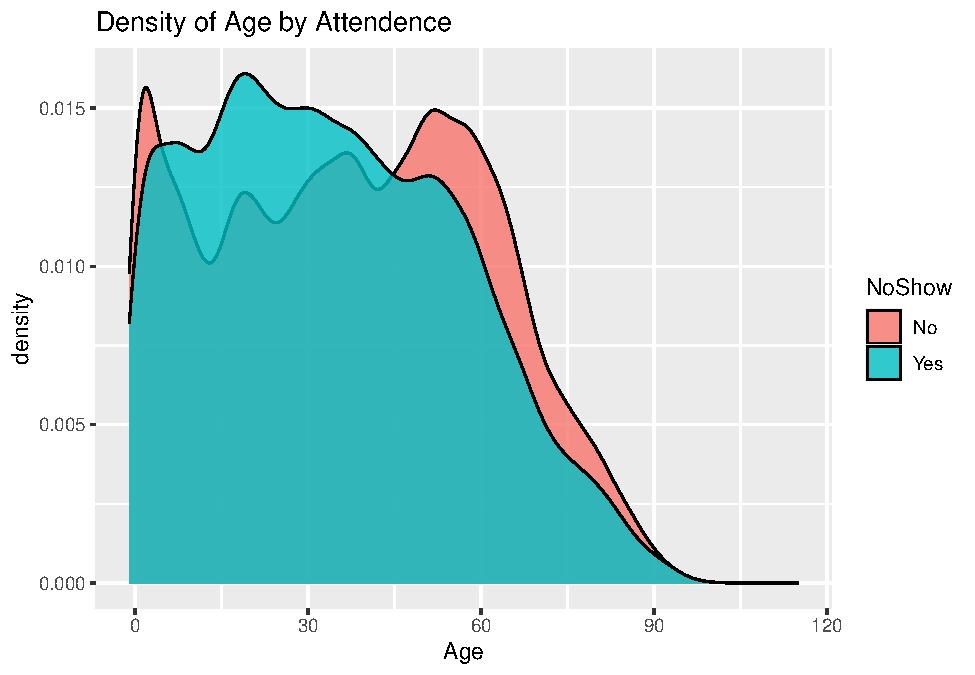
\includegraphics{lab1_medical_databases_files/figure-latex/unnamed-chunk-6-1} \end{center}

There does seem to be a difference in the distribution of ages of people
that miss and don't miss appointments.\\
However, the shape of this distribution means the actual correlation is
near 0 in the heatmap above. This highlights the need to look at
individual variables.

Let's take a closer look at age by breaking it into categories.

\begin{Shaded}
\begin{Highlighting}[]
\NormalTok{raw.data }\OtherTok{\textless{}{-}}\NormalTok{ raw.data }\SpecialCharTok{\%\textgreater{}\%} \FunctionTok{mutate}\NormalTok{(}\AttributeTok{Age.Range=}\FunctionTok{cut\_interval}\NormalTok{(Age, }\AttributeTok{length=}\DecValTok{10}\NormalTok{))}

\FunctionTok{ggplot}\NormalTok{(raw.data) }\SpecialCharTok{+} 
  \FunctionTok{geom\_bar}\NormalTok{(}\FunctionTok{aes}\NormalTok{(}\AttributeTok{x=}\NormalTok{Age.Range, }\AttributeTok{fill=}\NormalTok{NoShow)) }\SpecialCharTok{+} 
  \FunctionTok{ggtitle}\NormalTok{(}\StringTok{"Amount of No Show across Age Ranges"}\NormalTok{)}
\end{Highlighting}
\end{Shaded}

\begin{center}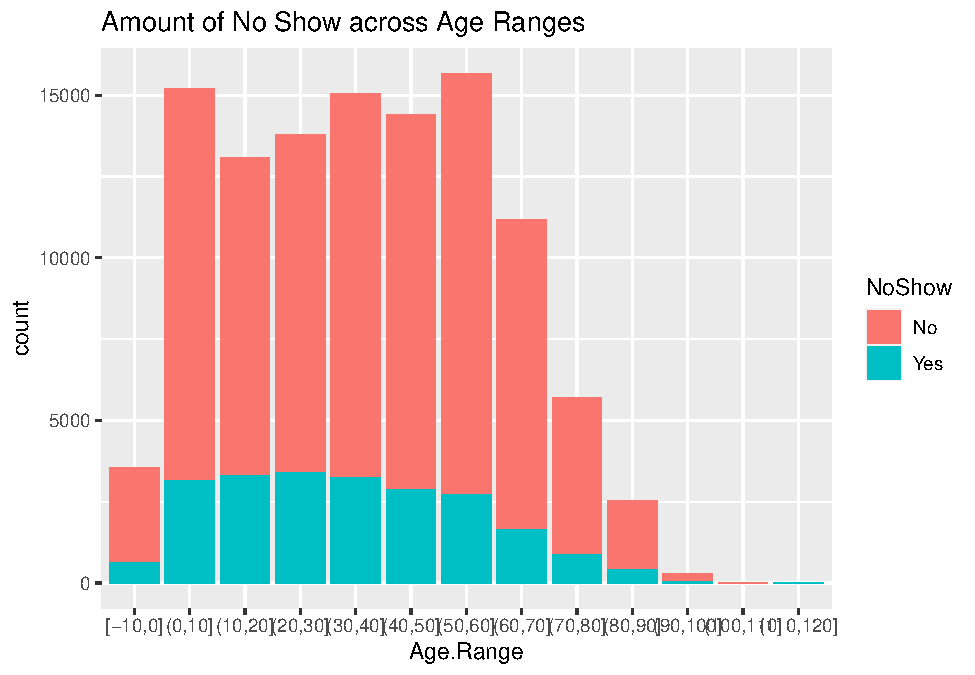
\includegraphics{lab1_medical_databases_files/figure-latex/unnamed-chunk-7-1} \end{center}

\begin{Shaded}
\begin{Highlighting}[]
\FunctionTok{ggplot}\NormalTok{(raw.data) }\SpecialCharTok{+} 
  \FunctionTok{geom\_bar}\NormalTok{(}\FunctionTok{aes}\NormalTok{(}\AttributeTok{x=}\NormalTok{Age.Range, }\AttributeTok{fill=}\NormalTok{NoShow), }\AttributeTok{position=}\StringTok{\textquotesingle{}fill\textquotesingle{}}\NormalTok{) }\SpecialCharTok{+} 
  \FunctionTok{ggtitle}\NormalTok{(}\StringTok{"Proportion of No Show across Age Ranges"}\NormalTok{)}
\end{Highlighting}
\end{Shaded}

\begin{center}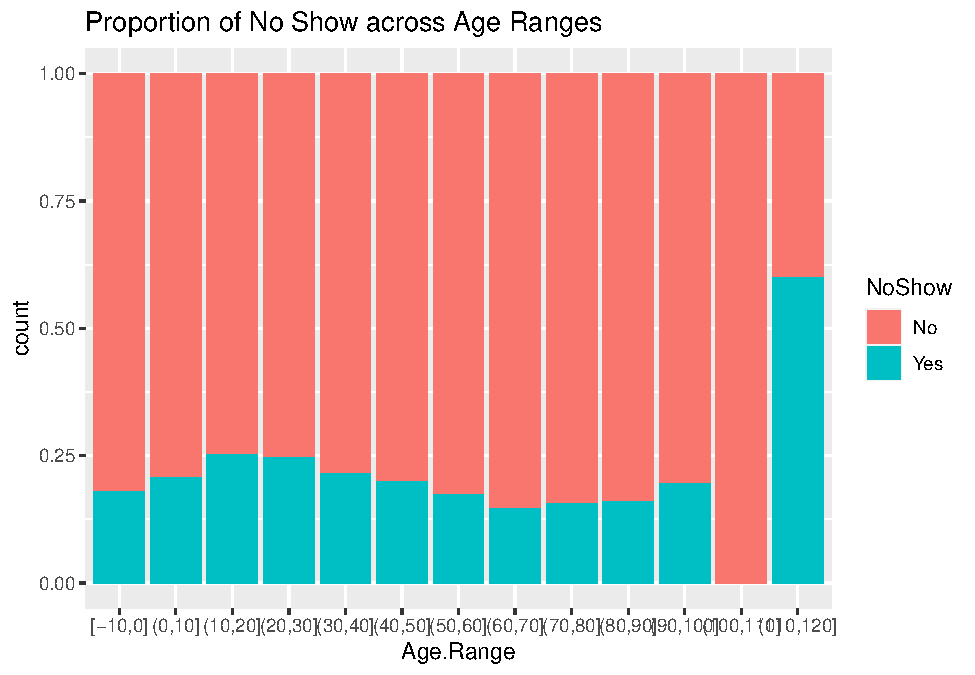
\includegraphics{lab1_medical_databases_files/figure-latex/unnamed-chunk-7-2} \end{center}

\textbf{10} How could you be misled if you only plotted 1 of these 2
plots of attendance by age group?

You could be misled if you only plotted 1 of these 2 plots of attendance
by age group because 1 plot is showing counts and one plot is showing
proportions. In plot 1, it looks as if individuals aged 0 to 30 have the
most no shows, and no shows decrease with age, since there are very few
individuals over 90. In plot 2, it looks as if individuals aged 10 to 30
have the most no shows and decreases with age until 60, then increases
rapidly as there is a smaller number of older individuals, but there is
a larger proportion of no shows here. There are very few individuals
older than 90 years old from plot 1, therefore this does not really
impact the overall distributions. There are twice as many missed
appointments in the 10-20 age group compared to the 60-70 age group. The
zero age group has some no shows since the observations with missing age
will be in that category.

\begin{Shaded}
\begin{Highlighting}[]
\NormalTok{raw.data }\SpecialCharTok{\%\textgreater{}\%} \FunctionTok{filter}\NormalTok{(Age }\SpecialCharTok{==} \DecValTok{0}\NormalTok{) }\SpecialCharTok{\%\textgreater{}\%} \FunctionTok{count}\NormalTok{()}
\end{Highlighting}
\end{Shaded}

\begin{verbatim}
## # A tibble: 1 x 1
##       n
##   <int>
## 1  3539
\end{verbatim}

Next, we'll have a look at \texttt{SMSReceived} variable:

\begin{Shaded}
\begin{Highlighting}[]
\FunctionTok{ggplot}\NormalTok{(raw.data) }\SpecialCharTok{+} 
  \FunctionTok{geom\_bar}\NormalTok{(}\FunctionTok{aes}\NormalTok{(}\AttributeTok{x=}\NormalTok{SMSReceived, }\AttributeTok{fill=}\NormalTok{NoShow), }\AttributeTok{alpha=}\FloatTok{0.8}\NormalTok{) }\SpecialCharTok{+} 
  \FunctionTok{ggtitle}\NormalTok{(}\StringTok{"Density of SMS received across Age and No Show"}\NormalTok{)}
\end{Highlighting}
\end{Shaded}

\begin{center}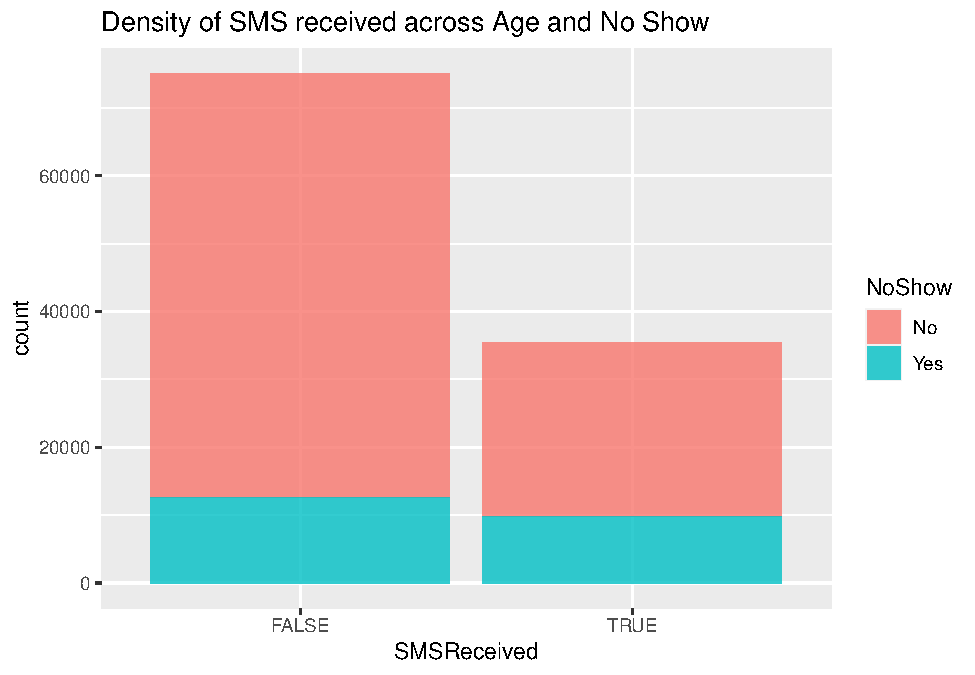
\includegraphics{lab1_medical_databases_files/figure-latex/unnamed-chunk-9-1} \end{center}

\begin{Shaded}
\begin{Highlighting}[]
\FunctionTok{ggplot}\NormalTok{(raw.data) }\SpecialCharTok{+} 
  \FunctionTok{geom\_bar}\NormalTok{(}\FunctionTok{aes}\NormalTok{(}\AttributeTok{x=}\NormalTok{SMSReceived, }\AttributeTok{fill=}\NormalTok{NoShow), }\AttributeTok{position=}\StringTok{\textquotesingle{}fill\textquotesingle{}}\NormalTok{, }\AttributeTok{alpha=}\FloatTok{0.8}\NormalTok{) }\SpecialCharTok{+} 
  \FunctionTok{ggtitle}\NormalTok{(}\StringTok{"Density of SMS received across Age and No Show"}\NormalTok{)}
\end{Highlighting}
\end{Shaded}

\begin{center}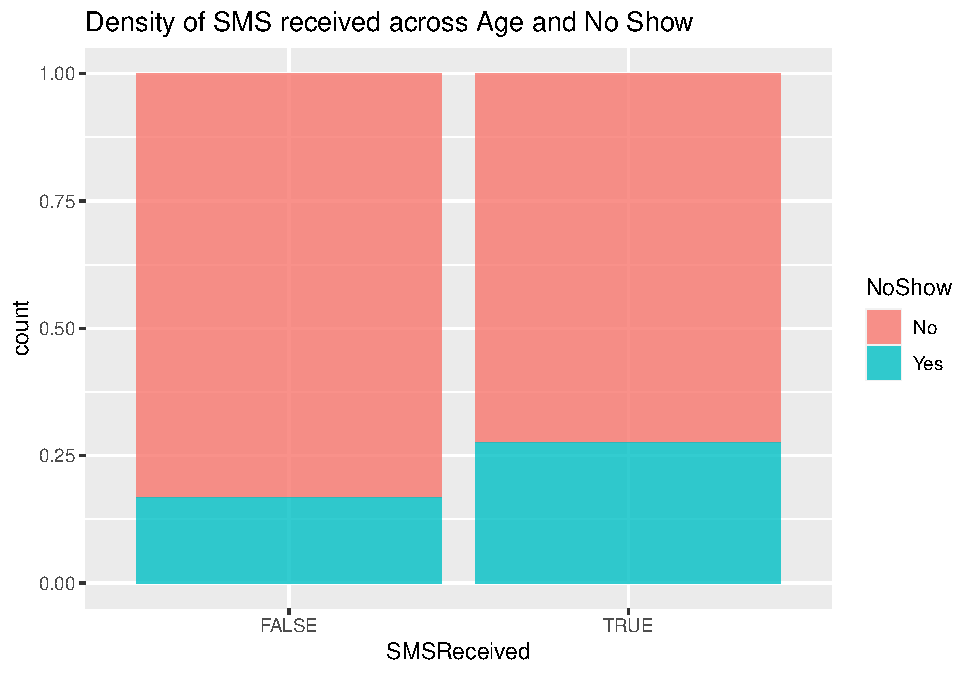
\includegraphics{lab1_medical_databases_files/figure-latex/unnamed-chunk-9-2} \end{center}

\textbf{11} From this plot does it look like SMS reminders increase or
decrease the chance of someone not attending an appointment? Why might
the opposite actually be true (hint: think about biases)?

From the plot it does look like SMS reminders increase the chance of
someone not attending an appointment. This could be the case because
individuals who have same day or walk-in appointments may not be
receiving a text message reminder, and they do show up. This would make
the SMS Received FALSE. This could also be biased because older
individuals may be less likely to have cell phones, and therefore may
not be able to receive text messages, which would therefore make the SMS
Received variable FALSE.

Therefore the individuals that do not received a SMS reminder may be
more likely to show up to their appointment since it may be on the same
day or they just do not have a cell phone. This is biased according to
the plot and thats why the opposite (individuals that do not received a
SMS reminder may be more likely to show up to their appointment) may be
true.

\textbf{12} Create a similar plot which compares the the density of
\texttt{NoShow} across the values of disability

\begin{Shaded}
\begin{Highlighting}[]
\FunctionTok{ggplot}\NormalTok{(raw.data) }\SpecialCharTok{+} 
  \FunctionTok{geom\_bar}\NormalTok{(}\FunctionTok{aes}\NormalTok{(}\AttributeTok{x=}\NormalTok{Disability, }\AttributeTok{fill=}\NormalTok{NoShow), }\AttributeTok{alpha=}\FloatTok{0.8}\NormalTok{) }\SpecialCharTok{+} 
  \FunctionTok{ggtitle}\NormalTok{(}\StringTok{"Density of SMS received across Disability and No Show"}\NormalTok{)}
\end{Highlighting}
\end{Shaded}

\begin{center}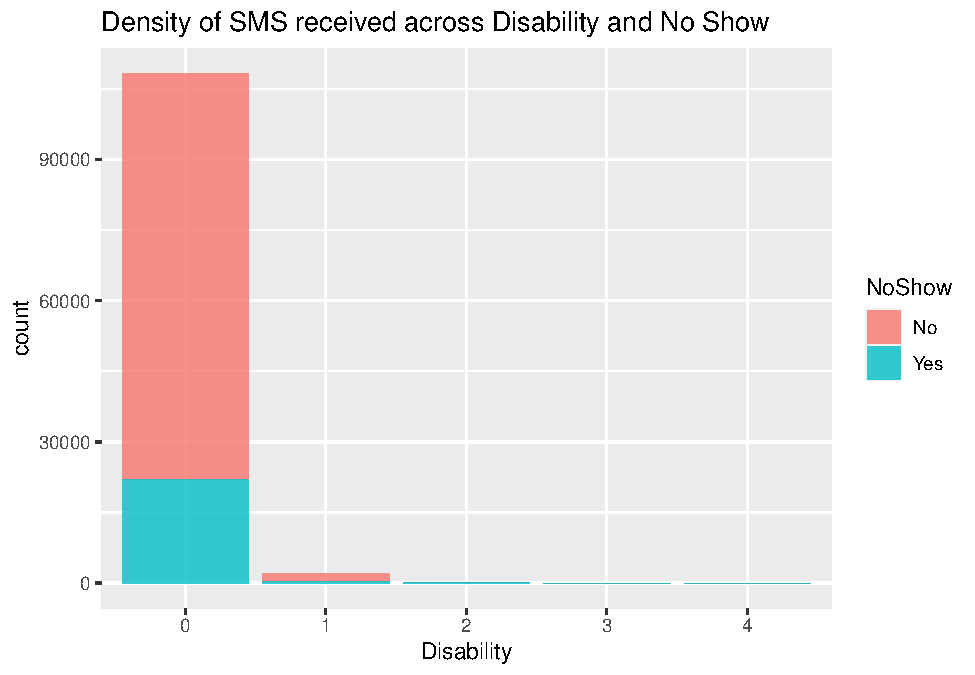
\includegraphics{lab1_medical_databases_files/figure-latex/unnamed-chunk-10-1} \end{center}

\begin{Shaded}
\begin{Highlighting}[]
\FunctionTok{ggplot}\NormalTok{(raw.data) }\SpecialCharTok{+} 
  \FunctionTok{geom\_bar}\NormalTok{(}\FunctionTok{aes}\NormalTok{(}\AttributeTok{x=}\NormalTok{Disability, }\AttributeTok{fill=}\NormalTok{NoShow), }\AttributeTok{position=}\StringTok{\textquotesingle{}fill\textquotesingle{}}\NormalTok{, }\AttributeTok{alpha=}\FloatTok{0.8}\NormalTok{) }\SpecialCharTok{+} 
  \FunctionTok{ggtitle}\NormalTok{(}\StringTok{"Density of SMS received across Disability and No Show"}\NormalTok{)}
\end{Highlighting}
\end{Shaded}

\begin{center}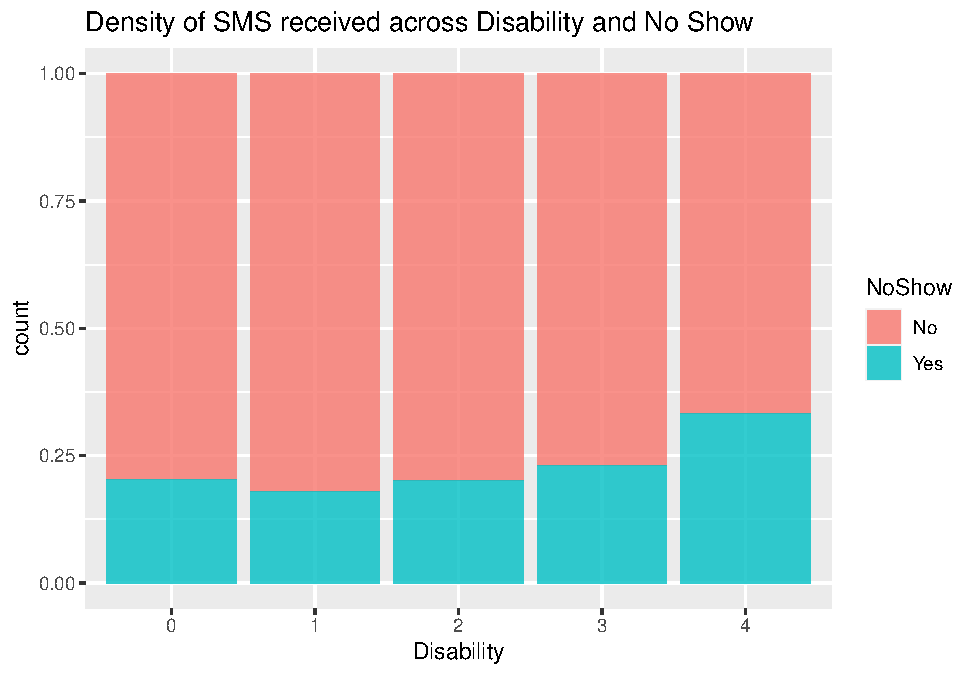
\includegraphics{lab1_medical_databases_files/figure-latex/unnamed-chunk-10-2} \end{center}

Now let's look at the neighbourhood data as location can correlate
highly with many social determinants of health.

\begin{Shaded}
\begin{Highlighting}[]
\FunctionTok{ggplot}\NormalTok{(raw.data) }\SpecialCharTok{+} 
  \FunctionTok{geom\_bar}\NormalTok{(}\FunctionTok{aes}\NormalTok{(}\AttributeTok{x=}\NormalTok{Neighbourhood, }\AttributeTok{fill=}\NormalTok{NoShow)) }\SpecialCharTok{+} 
  \FunctionTok{theme}\NormalTok{(}\AttributeTok{axis.text.x =} \FunctionTok{element\_text}\NormalTok{(}\AttributeTok{angle=}\DecValTok{45}\NormalTok{, }\AttributeTok{hjust=}\DecValTok{1}\NormalTok{, }\AttributeTok{size=}\DecValTok{5}\NormalTok{)) }\SpecialCharTok{+} 
  \FunctionTok{ggtitle}\NormalTok{(}\StringTok{\textquotesingle{}Attendance by Neighbourhood\textquotesingle{}}\NormalTok{)}
\end{Highlighting}
\end{Shaded}

\begin{center}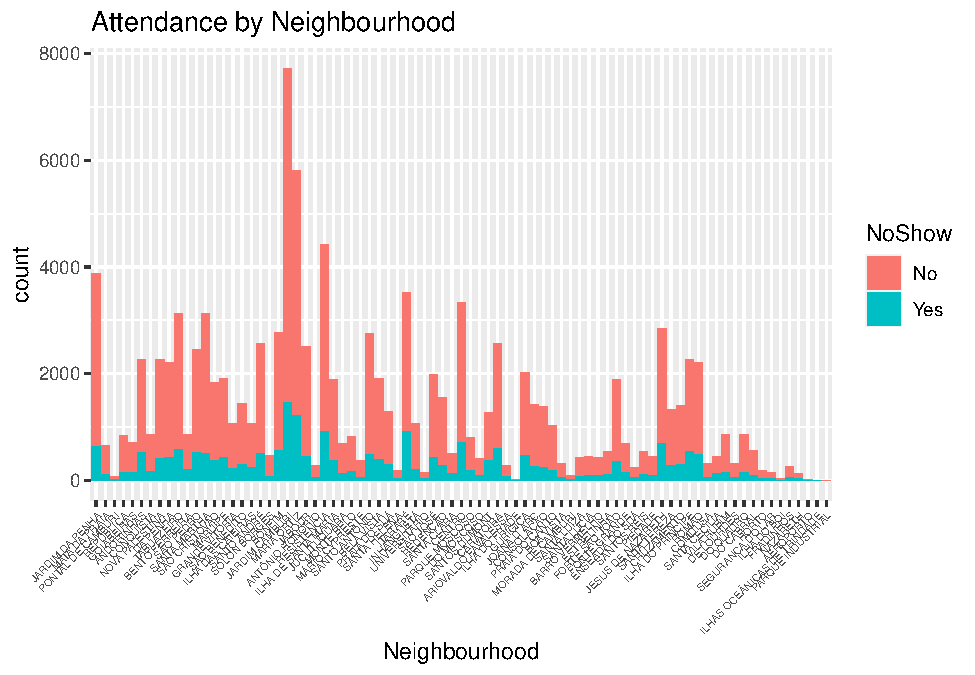
\includegraphics{lab1_medical_databases_files/figure-latex/unnamed-chunk-11-1} \end{center}

\begin{Shaded}
\begin{Highlighting}[]
\FunctionTok{ggplot}\NormalTok{(raw.data) }\SpecialCharTok{+} 
  \FunctionTok{geom\_bar}\NormalTok{(}\FunctionTok{aes}\NormalTok{(}\AttributeTok{x=}\NormalTok{Neighbourhood, }\AttributeTok{fill=}\NormalTok{NoShow), }\AttributeTok{position=}\StringTok{\textquotesingle{}fill\textquotesingle{}}\NormalTok{) }\SpecialCharTok{+} 
  \FunctionTok{theme}\NormalTok{(}\AttributeTok{axis.text.x =} \FunctionTok{element\_text}\NormalTok{(}\AttributeTok{angle=}\DecValTok{45}\NormalTok{, }\AttributeTok{hjust=}\DecValTok{1}\NormalTok{, }\AttributeTok{size=}\DecValTok{5}\NormalTok{)) }\SpecialCharTok{+} 
  \FunctionTok{ggtitle}\NormalTok{(}\StringTok{\textquotesingle{}Proportional Attendance by Neighbourhood\textquotesingle{}}\NormalTok{)}
\end{Highlighting}
\end{Shaded}

\begin{center}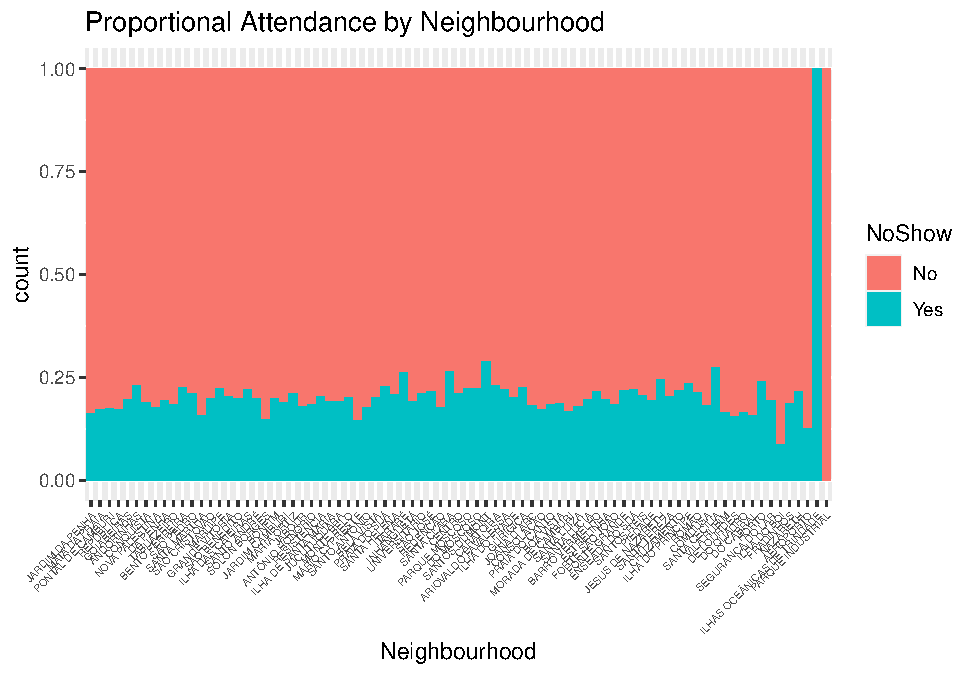
\includegraphics{lab1_medical_databases_files/figure-latex/unnamed-chunk-11-2} \end{center}

Most neighborhoods have similar proportions of no-show but some have
much higher and lower rates.

\textbf{13} Suggest a reason for differences in attendance rates across
neighbourhoods.

A possible reason for differences in attendance rates across
neighborhoods could be differences in socioeconomic status or distance
from appointment site. If individuals are from a certain low SES
neighborhood then they may not have access to a car and this could be a
barrier to overcome when getting to their appointment. Individuals that
live in a certain neighborhood that is really far away from the
appointment site may be less likely to get to their appointment due to
the time it takes to get their (due to traffic, etc.).

Now let's explore the relationship between gender and NoShow.

\begin{Shaded}
\begin{Highlighting}[]
\FunctionTok{ggplot}\NormalTok{(raw.data) }\SpecialCharTok{+} 
  \FunctionTok{geom\_bar}\NormalTok{(}\FunctionTok{aes}\NormalTok{(}\AttributeTok{x=}\NormalTok{Gender, }\AttributeTok{fill=}\NormalTok{NoShow))}
\end{Highlighting}
\end{Shaded}

\begin{center}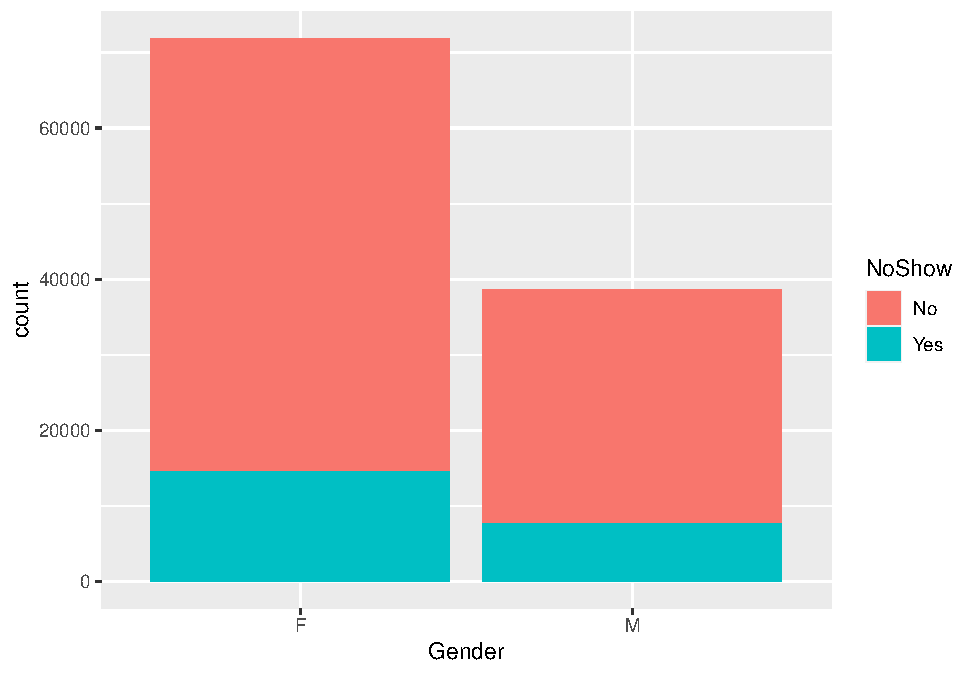
\includegraphics{lab1_medical_databases_files/figure-latex/unnamed-chunk-12-1} \end{center}

\begin{Shaded}
\begin{Highlighting}[]
  \FunctionTok{ggtitle}\NormalTok{(}\StringTok{"Gender by attendance"}\NormalTok{)}
\end{Highlighting}
\end{Shaded}

\begin{verbatim}
## $title
## [1] "Gender by attendance"
## 
## attr(,"class")
## [1] "labels"
\end{verbatim}

\begin{Shaded}
\begin{Highlighting}[]
\FunctionTok{ggplot}\NormalTok{(raw.data) }\SpecialCharTok{+} 
  \FunctionTok{geom\_bar}\NormalTok{(}\FunctionTok{aes}\NormalTok{(}\AttributeTok{x=}\NormalTok{Gender, }\AttributeTok{fill=}\NormalTok{NoShow), }\AttributeTok{position=}\StringTok{\textquotesingle{}fill\textquotesingle{}}\NormalTok{)}
\end{Highlighting}
\end{Shaded}

\begin{center}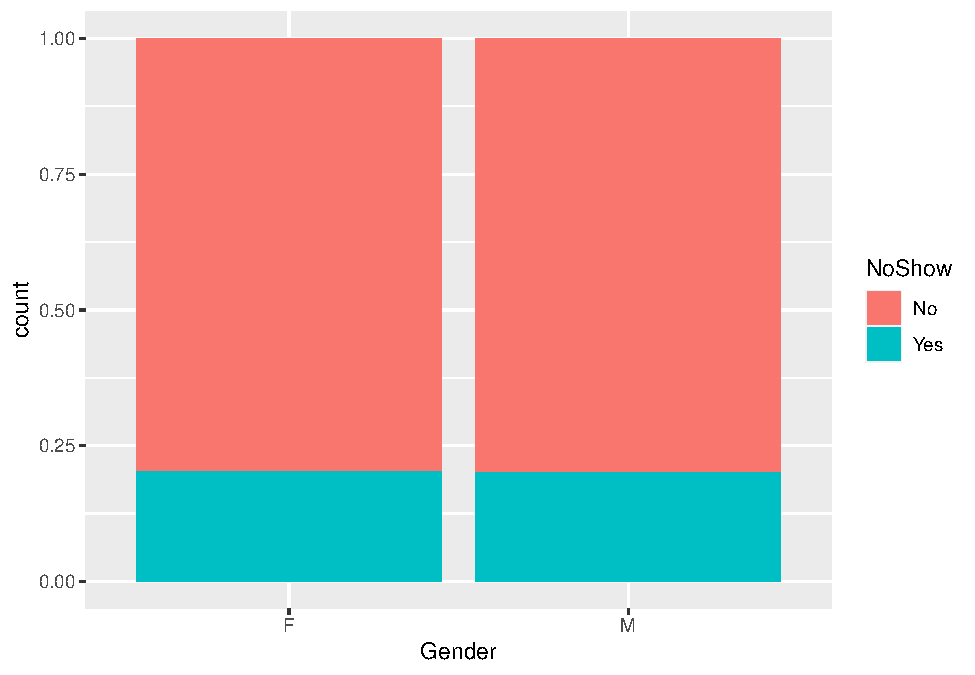
\includegraphics{lab1_medical_databases_files/figure-latex/unnamed-chunk-12-2} \end{center}

\begin{Shaded}
\begin{Highlighting}[]
  \FunctionTok{ggtitle}\NormalTok{(}\StringTok{"Gender by attendance"}\NormalTok{)}
\end{Highlighting}
\end{Shaded}

\begin{verbatim}
## $title
## [1] "Gender by attendance"
## 
## attr(,"class")
## [1] "labels"
\end{verbatim}

\textbf{14} Create a similar plot using \texttt{SocialWelfare}

\begin{Shaded}
\begin{Highlighting}[]
\FunctionTok{ggplot}\NormalTok{(raw.data) }\SpecialCharTok{+} 
  \FunctionTok{geom\_bar}\NormalTok{(}\FunctionTok{aes}\NormalTok{(}\AttributeTok{x=}\NormalTok{SocialWelfare, }\AttributeTok{fill=}\NormalTok{NoShow))}
\end{Highlighting}
\end{Shaded}

\begin{center}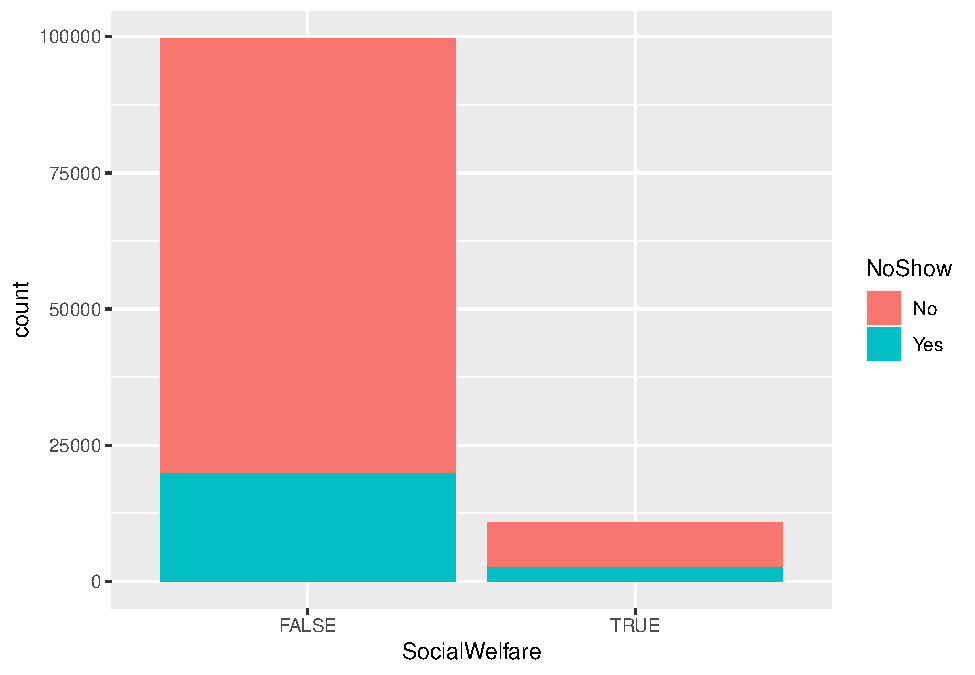
\includegraphics{lab1_medical_databases_files/figure-latex/unnamed-chunk-13-1} \end{center}

\begin{Shaded}
\begin{Highlighting}[]
  \FunctionTok{ggtitle}\NormalTok{(}\StringTok{"Social Welfare by attendance"}\NormalTok{)}
\end{Highlighting}
\end{Shaded}

\begin{verbatim}
## $title
## [1] "Social Welfare by attendance"
## 
## attr(,"class")
## [1] "labels"
\end{verbatim}

\begin{Shaded}
\begin{Highlighting}[]
\FunctionTok{ggplot}\NormalTok{(raw.data) }\SpecialCharTok{+} 
  \FunctionTok{geom\_bar}\NormalTok{(}\FunctionTok{aes}\NormalTok{(}\AttributeTok{x=}\NormalTok{SocialWelfare, }\AttributeTok{fill=}\NormalTok{NoShow), }\AttributeTok{position=}\StringTok{\textquotesingle{}fill\textquotesingle{}}\NormalTok{)}
\end{Highlighting}
\end{Shaded}

\begin{center}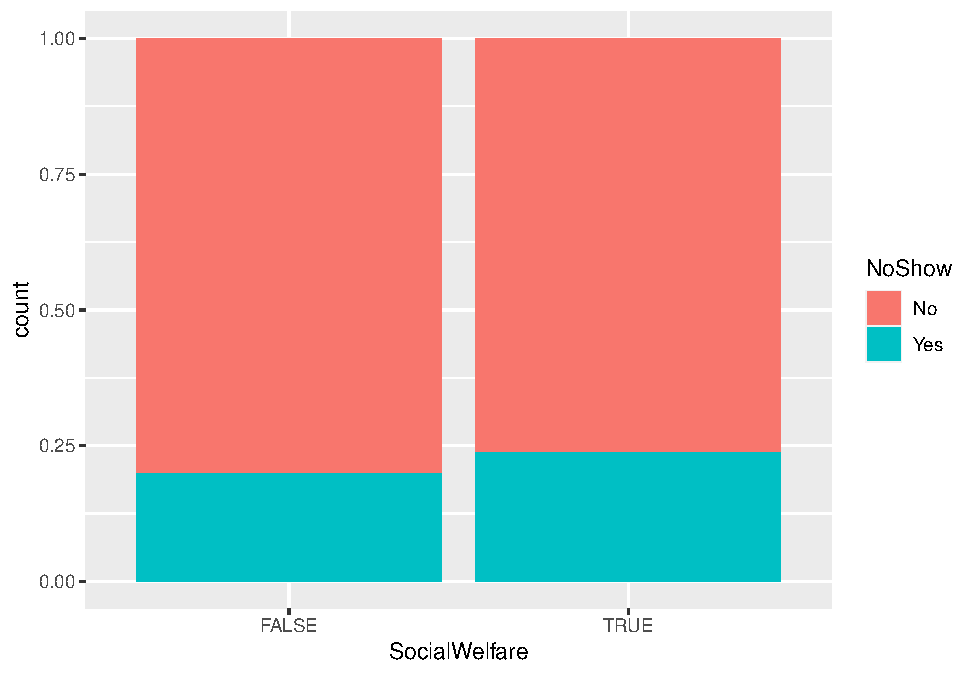
\includegraphics{lab1_medical_databases_files/figure-latex/unnamed-chunk-13-2} \end{center}

\begin{Shaded}
\begin{Highlighting}[]
  \FunctionTok{ggtitle}\NormalTok{(}\StringTok{"Social Welfare by attendance"}\NormalTok{)}
\end{Highlighting}
\end{Shaded}

\begin{verbatim}
## $title
## [1] "Social Welfare by attendance"
## 
## attr(,"class")
## [1] "labels"
\end{verbatim}

Far more exploration could still be done, including dimensionality
reduction approaches but although we have found some patterns there is
no major/striking patterns on the data as it currently stands.

However, maybe we can generate some new features/variables that more
strongly relate to the \texttt{NoShow}.

\hypertarget{feature-engineering}{%
\subsection{Feature Engineering}\label{feature-engineering}}

Let's begin by seeing if appointments on any day of the week has more
no-show's. Fortunately, the \texttt{lubridate} library makes this quite
easy!

\begin{Shaded}
\begin{Highlighting}[]
\NormalTok{raw.data }\OtherTok{\textless{}{-}}\NormalTok{ raw.data }\SpecialCharTok{\%\textgreater{}\%} \FunctionTok{mutate}\NormalTok{(}\AttributeTok{AppointmentDay =} \FunctionTok{wday}\NormalTok{(AppointmentDate, }\AttributeTok{label=}\ConstantTok{TRUE}\NormalTok{, }\AttributeTok{abbr=}\ConstantTok{TRUE}\NormalTok{), }
                                 \AttributeTok{ScheduledDay =} \FunctionTok{wday}\NormalTok{(ScheduledDate,  }\AttributeTok{label=}\ConstantTok{TRUE}\NormalTok{, }\AttributeTok{abbr=}\ConstantTok{TRUE}\NormalTok{))}

\FunctionTok{ggplot}\NormalTok{(raw.data) }\SpecialCharTok{+}
  \FunctionTok{geom\_bar}\NormalTok{(}\FunctionTok{aes}\NormalTok{(}\AttributeTok{x=}\NormalTok{AppointmentDay, }\AttributeTok{fill=}\NormalTok{NoShow)) }\SpecialCharTok{+}
  \FunctionTok{ggtitle}\NormalTok{(}\StringTok{"Amount of No Show across Appointment Day"}\NormalTok{) }
\end{Highlighting}
\end{Shaded}

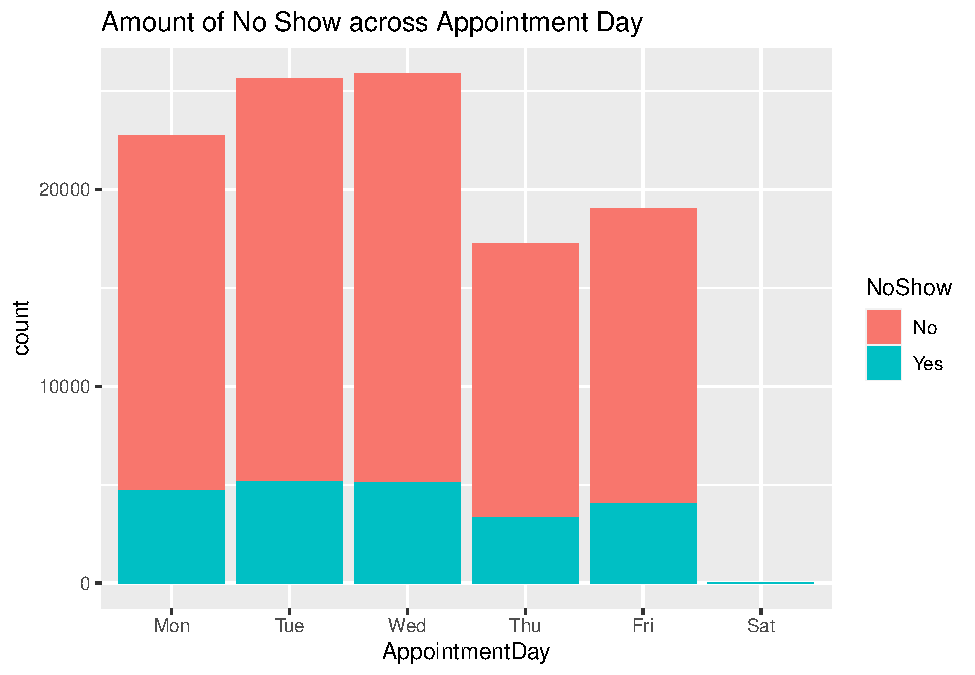
\includegraphics{lab1_medical_databases_files/figure-latex/unnamed-chunk-14-1.pdf}

\begin{Shaded}
\begin{Highlighting}[]
\FunctionTok{ggplot}\NormalTok{(raw.data) }\SpecialCharTok{+}
  \FunctionTok{geom\_bar}\NormalTok{(}\FunctionTok{aes}\NormalTok{(}\AttributeTok{x=}\NormalTok{AppointmentDay, }\AttributeTok{fill=}\NormalTok{NoShow), }\AttributeTok{position =} \StringTok{\textquotesingle{}fill\textquotesingle{}}\NormalTok{) }\SpecialCharTok{+}
  \FunctionTok{ggtitle}\NormalTok{(}\StringTok{"Amount of No Show across Appointment Day"}\NormalTok{) }
\end{Highlighting}
\end{Shaded}

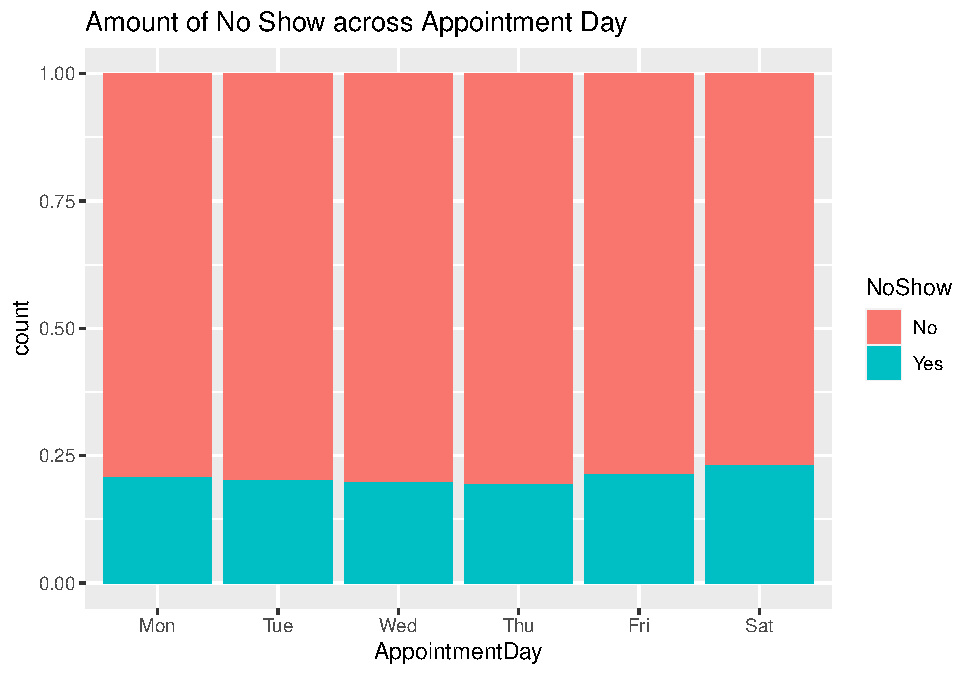
\includegraphics{lab1_medical_databases_files/figure-latex/unnamed-chunk-14-2.pdf}
Let's begin by creating a variable called \texttt{Lag}, which is the
difference between when an appointment was scheduled and the actual
appointment.

\begin{Shaded}
\begin{Highlighting}[]
\NormalTok{raw.data }\OtherTok{\textless{}{-}}\NormalTok{ raw.data }\SpecialCharTok{\%\textgreater{}\%} \FunctionTok{mutate}\NormalTok{(}\AttributeTok{Lag.days=}\FunctionTok{difftime}\NormalTok{(AppointmentDate, ScheduledDate, }\AttributeTok{units =} \StringTok{"days"}\NormalTok{),}
                                \AttributeTok{Lag.hours=}\FunctionTok{difftime}\NormalTok{(AppointmentDate, ScheduledDate, }\AttributeTok{units =} \StringTok{"hours"}\NormalTok{))}

\FunctionTok{ggplot}\NormalTok{(raw.data) }\SpecialCharTok{+} 
  \FunctionTok{geom\_density}\NormalTok{(}\FunctionTok{aes}\NormalTok{(}\AttributeTok{x=}\NormalTok{Lag.days, }\AttributeTok{fill=}\NormalTok{NoShow), }\AttributeTok{alpha=}\FloatTok{0.7}\NormalTok{)}\SpecialCharTok{+}
  \FunctionTok{ggtitle}\NormalTok{(}\StringTok{"Density of Lag (days) by attendance"}\NormalTok{)}
\end{Highlighting}
\end{Shaded}

\begin{verbatim}
## Don't know how to automatically pick scale for object of type <difftime>.
## Defaulting to continuous.
\end{verbatim}

\begin{center}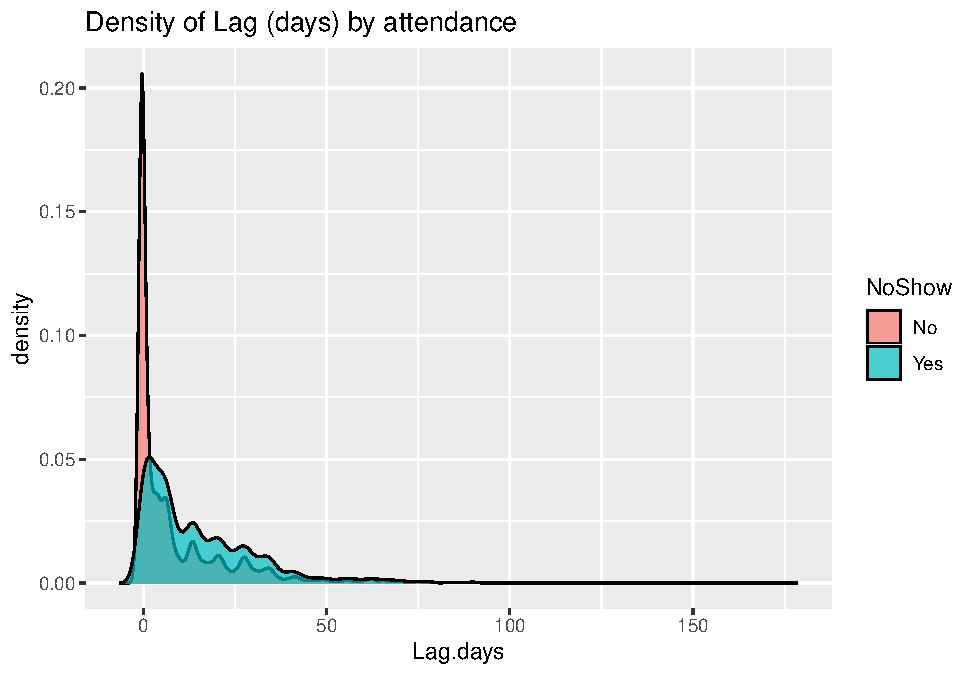
\includegraphics{lab1_medical_databases_files/figure-latex/unnamed-chunk-15-1} \end{center}

\textbf{15} Have a look at the values in lag variable, does anything
seem odd?

In the graph, it does show that there are lag days that are less than
zero and there is a huge number of lag days that are zero. Negative lag
days means that the scheduled date was a later date than when the
appointment date was. This could be an error when entering the dates and
interpreting the days and months in reverse. When considering the lag
days that are zero, this could be appointments that are scheduled (or
individuals just show up) and occur on the same day; which could be walk
in appointments. When interpreting models, it will be necessary to
distinguish between walk in and scheduled appointments. Since these two
types of appointments are included here, it may be difficult to develop
a good prediction model.

\hypertarget{predictive-modeling}{%
\subsection{Predictive Modeling}\label{predictive-modeling}}

Let's see how well we can predict NoShow from the data.

We'll start by preparing the data, followed by splitting it into testing
and training set, modeling and finally, evaluating our results. For now
we will subsample but please run on full dataset for final execution.

\begin{Shaded}
\begin{Highlighting}[]
\DocumentationTok{\#\#\# REMOVE SUBSAMPLING FOR FINAL MODEL}
\NormalTok{data.prep }\OtherTok{\textless{}{-}}\NormalTok{ raw.data }\SpecialCharTok{\%\textgreater{}\%} \FunctionTok{select}\NormalTok{(}\SpecialCharTok{{-}}\NormalTok{AppointmentID, }\SpecialCharTok{{-}}\NormalTok{PatientID) }\CommentTok{\#\%\textgreater{}\% sample\_n(10000)}

\FunctionTok{set.seed}\NormalTok{(}\DecValTok{42}\NormalTok{)}
\NormalTok{data.split }\OtherTok{\textless{}{-}} \FunctionTok{initial\_split}\NormalTok{(data.prep, }\AttributeTok{prop =} \FloatTok{0.7}\NormalTok{)}
\NormalTok{train  }\OtherTok{\textless{}{-}} \FunctionTok{training}\NormalTok{(data.split)}
\NormalTok{test }\OtherTok{\textless{}{-}} \FunctionTok{testing}\NormalTok{(data.split)}
\end{Highlighting}
\end{Shaded}

Let's now set the cross validation parameters, and add classProbs so we
can use AUC as a metric for xgboost.

\begin{Shaded}
\begin{Highlighting}[]
\NormalTok{fit.control }\OtherTok{\textless{}{-}} \FunctionTok{trainControl}\NormalTok{(}\AttributeTok{method=}\StringTok{"cv"}\NormalTok{,}\AttributeTok{number=}\DecValTok{3}\NormalTok{,}
                           \AttributeTok{classProbs =} \ConstantTok{TRUE}\NormalTok{, }\AttributeTok{summaryFunction =}\NormalTok{ twoClassSummary)}
\end{Highlighting}
\end{Shaded}

\textbf{16} Based on the EDA, how well do you think this is going to
work?

Based on the exploratory data analysis, there have been some issues
identified. There are some important variables missing from the data set
when predicting no shows such as: distance from site, a more direct
identifier of income, and type of disability. The variables in the data
set may do a decent job of predicting no shows, but there could be more
options that could be better predictors of whether an individual will
not show up to their appointment. Another issue is that there are a few
outliers in the data set that are hard to distinguish if they are
biologically plausible or not. Keeping these individuals in the data set
may skew the results very slightly, but since there are 110 527
observations this should not be an issue, but should be considered.
There is a bias that was associated with SMS reminders that could impact
how well the prediction model will work. Prediction may also be
difficult since walk-in and scheduled appointments are being consdiered
here, based on the lag time variable. Therefore, based on the issues
mentioned above, this prediction model may not predict no shows very
well.

Now we can train our XGBoost model

\begin{Shaded}
\begin{Highlighting}[]
\NormalTok{xgb.grid }\OtherTok{\textless{}{-}} \FunctionTok{expand.grid}\NormalTok{(}\AttributeTok{eta=}\FunctionTok{c}\NormalTok{(}\FloatTok{0.05}\NormalTok{),}
                       \AttributeTok{max\_depth=}\FunctionTok{c}\NormalTok{(}\DecValTok{4}\NormalTok{),}\AttributeTok{colsample\_bytree=}\DecValTok{1}\NormalTok{,}
                       \AttributeTok{subsample=}\DecValTok{1}\NormalTok{, }\AttributeTok{nrounds=}\DecValTok{500}\NormalTok{, }\AttributeTok{gamma=}\DecValTok{0}\NormalTok{, }\AttributeTok{min\_child\_weight=}\DecValTok{5}\NormalTok{)}

\NormalTok{xgb.model }\OtherTok{\textless{}{-}} \FunctionTok{train}\NormalTok{(NoShow }\SpecialCharTok{\textasciitilde{}}\NormalTok{ .,}\AttributeTok{data=}\NormalTok{train, }\AttributeTok{method=}\StringTok{"xgbTree"}\NormalTok{,}\AttributeTok{metric=}\StringTok{"ROC"}\NormalTok{,}
                  \AttributeTok{tuneGrid=}\NormalTok{xgb.grid, }\AttributeTok{trControl=}\NormalTok{fit.control)}

\NormalTok{xgb.pred }\OtherTok{\textless{}{-}} \FunctionTok{predict}\NormalTok{(xgb.model, }\AttributeTok{newdata=}\NormalTok{test)}
\NormalTok{xgb.probs }\OtherTok{\textless{}{-}} \FunctionTok{predict}\NormalTok{(xgb.model, }\AttributeTok{newdata=}\NormalTok{test, }\AttributeTok{type=}\StringTok{"prob"}\NormalTok{)}
\end{Highlighting}
\end{Shaded}

\begin{Shaded}
\begin{Highlighting}[]
\NormalTok{test }\OtherTok{\textless{}{-}}\NormalTok{ test }\SpecialCharTok{\%\textgreater{}\%} \FunctionTok{mutate}\NormalTok{(}\AttributeTok{NoShow.numerical =} \FunctionTok{ifelse}\NormalTok{(NoShow}\SpecialCharTok{==}\StringTok{"Yes"}\NormalTok{,}\DecValTok{1}\NormalTok{,}\DecValTok{0}\NormalTok{))}
\FunctionTok{confusionMatrix}\NormalTok{(xgb.pred, test}\SpecialCharTok{$}\NormalTok{NoShow, }\AttributeTok{positive=}\StringTok{"Yes"}\NormalTok{)}
\end{Highlighting}
\end{Shaded}

\begin{verbatim}
## Confusion Matrix and Statistics
## 
##           Reference
## Prediction    No   Yes
##        No  26385  6390
##        Yes   142   242
##                                           
##                Accuracy : 0.803           
##                  95% CI : (0.7987, 0.8073)
##     No Information Rate : 0.8             
##     P-Value [Acc > NIR] : 0.08578         
##                                           
##                   Kappa : 0.0481          
##                                           
##  Mcnemar's Test P-Value : < 2e-16         
##                                           
##             Sensitivity : 0.036490        
##             Specificity : 0.994647        
##          Pos Pred Value : 0.630208        
##          Neg Pred Value : 0.805034        
##              Prevalence : 0.200006        
##          Detection Rate : 0.007298        
##    Detection Prevalence : 0.011581        
##       Balanced Accuracy : 0.515568        
##                                           
##        'Positive' Class : Yes             
## 
\end{verbatim}

\begin{Shaded}
\begin{Highlighting}[]
\FunctionTok{paste}\NormalTok{(}\StringTok{"XGBoost Area under ROC Curve: "}\NormalTok{, }\FunctionTok{round}\NormalTok{(}\FunctionTok{auc}\NormalTok{(test}\SpecialCharTok{$}\NormalTok{NoShow.numerical, xgb.probs[,}\DecValTok{2}\NormalTok{]),}\DecValTok{3}\NormalTok{), }\AttributeTok{sep=}\StringTok{""}\NormalTok{)}
\end{Highlighting}
\end{Shaded}

\begin{verbatim}
## Setting levels: control = 0, case = 1
\end{verbatim}

\begin{verbatim}
## Setting direction: controls < cases
\end{verbatim}

\begin{verbatim}
## [1] "XGBoost Area under ROC Curve: 0.74"
\end{verbatim}

This isn't an unreasonable performance, but let's look a bit more
carefully at the correct and incorrect predictions,

\begin{Shaded}
\begin{Highlighting}[]
\NormalTok{xgb.probs}\SpecialCharTok{$}\NormalTok{Actual }\OtherTok{=}\NormalTok{ test}\SpecialCharTok{$}\NormalTok{NoShow.numerical}
\NormalTok{xgb.probs}\SpecialCharTok{$}\NormalTok{ActualClass }\OtherTok{=}\NormalTok{ test}\SpecialCharTok{$}\NormalTok{NoShow}
\NormalTok{xgb.probs}\SpecialCharTok{$}\NormalTok{PredictedClass }\OtherTok{=}\NormalTok{ xgb.pred}
\NormalTok{xgb.probs}\SpecialCharTok{$}\NormalTok{Match }\OtherTok{=} \FunctionTok{ifelse}\NormalTok{(xgb.probs}\SpecialCharTok{$}\NormalTok{ActualClass }\SpecialCharTok{==}\NormalTok{ xgb.probs}\SpecialCharTok{$}\NormalTok{PredictedClass,}
                         \StringTok{"Correct"}\NormalTok{,}\StringTok{"Incorrect"}\NormalTok{)}
\CommentTok{\# [4.8] Plot Accuracy}
\NormalTok{xgb.probs}\SpecialCharTok{$}\NormalTok{Match }\OtherTok{=} \FunctionTok{factor}\NormalTok{(xgb.probs}\SpecialCharTok{$}\NormalTok{Match,}\AttributeTok{levels=}\FunctionTok{c}\NormalTok{(}\StringTok{"Incorrect"}\NormalTok{,}\StringTok{"Correct"}\NormalTok{))}
\FunctionTok{ggplot}\NormalTok{(xgb.probs,}\FunctionTok{aes}\NormalTok{(}\AttributeTok{x=}\NormalTok{Yes,}\AttributeTok{y=}\NormalTok{Actual,}\AttributeTok{color=}\NormalTok{Match))}\SpecialCharTok{+}
  \FunctionTok{geom\_jitter}\NormalTok{(}\AttributeTok{alpha=}\FloatTok{0.2}\NormalTok{,}\AttributeTok{size=}\FloatTok{0.25}\NormalTok{)}\SpecialCharTok{+}
  \FunctionTok{scale\_color\_manual}\NormalTok{(}\AttributeTok{values=}\FunctionTok{c}\NormalTok{(}\StringTok{"grey40"}\NormalTok{,}\StringTok{"orangered"}\NormalTok{))}\SpecialCharTok{+}
  \FunctionTok{ggtitle}\NormalTok{(}\StringTok{"Visualizing Model Performance"}\NormalTok{, }\StringTok{"(Dust Plot)"}\NormalTok{)}
\end{Highlighting}
\end{Shaded}

\begin{center}\includegraphics{lab1_medical_databases_files/figure-latex/unnamed-chunk-20-1} \end{center}

Finally, let's close it off with the variable importance of our model:

\begin{Shaded}
\begin{Highlighting}[]
\NormalTok{results }\OtherTok{=} \FunctionTok{data.frame}\NormalTok{(}\AttributeTok{Feature =} \FunctionTok{rownames}\NormalTok{(}\FunctionTok{varImp}\NormalTok{(xgb.model)}\SpecialCharTok{$}\NormalTok{importance)[}\DecValTok{1}\SpecialCharTok{:}\DecValTok{10}\NormalTok{],}
                     \AttributeTok{Importance =} \FunctionTok{varImp}\NormalTok{(xgb.model)}\SpecialCharTok{$}\NormalTok{importance[}\DecValTok{1}\SpecialCharTok{:}\DecValTok{10}\NormalTok{,])}

\NormalTok{results}\SpecialCharTok{$}\NormalTok{Feature }\OtherTok{=} \FunctionTok{factor}\NormalTok{(results}\SpecialCharTok{$}\NormalTok{Feature,}\AttributeTok{levels=}\NormalTok{results}\SpecialCharTok{$}\NormalTok{Feature)}


\CommentTok{\# [4.10] Plot Variable Importance}
\FunctionTok{ggplot}\NormalTok{(results, }\FunctionTok{aes}\NormalTok{(}\AttributeTok{x=}\NormalTok{Feature, }\AttributeTok{y=}\NormalTok{Importance,}\AttributeTok{fill=}\NormalTok{Importance))}\SpecialCharTok{+}
  \FunctionTok{geom\_bar}\NormalTok{(}\AttributeTok{stat=}\StringTok{"identity"}\NormalTok{)}\SpecialCharTok{+}
  \FunctionTok{scale\_fill\_gradient}\NormalTok{(}\AttributeTok{low=}\StringTok{"grey20"}\NormalTok{,}\AttributeTok{high=}\StringTok{"orangered"}\NormalTok{)}\SpecialCharTok{+}
  \FunctionTok{ggtitle}\NormalTok{(}\StringTok{"XGBoost Variable Importance"}\NormalTok{)}\SpecialCharTok{+}
  \FunctionTok{theme}\NormalTok{(}\AttributeTok{axis.text.x =} \FunctionTok{element\_text}\NormalTok{(}\AttributeTok{angle =} \DecValTok{45}\NormalTok{, }\AttributeTok{hjust =} \DecValTok{1}\NormalTok{))}
\end{Highlighting}
\end{Shaded}

\begin{center}\includegraphics{lab1_medical_databases_files/figure-latex/unnamed-chunk-21-1} \end{center}

\textbf{17} Using the \href{https://topepo.github.io/caret/}{caret
package} fit and evaluate 1 other ML model on this data.

\begin{Shaded}
\begin{Highlighting}[]
\DocumentationTok{\#\#\# REMOVE SUBSAMPLING FOR FINAL MODEL}
\NormalTok{data.prep }\OtherTok{\textless{}{-}}\NormalTok{ raw.data }\SpecialCharTok{\%\textgreater{}\%} \FunctionTok{select}\NormalTok{(}\SpecialCharTok{{-}}\NormalTok{AppointmentID, }\SpecialCharTok{{-}}\NormalTok{PatientID) }\CommentTok{\#\%\textgreater{}\% sample\_n(10000)}

\FunctionTok{set.seed}\NormalTok{(}\DecValTok{42}\NormalTok{)}
\NormalTok{data.split }\OtherTok{\textless{}{-}} \FunctionTok{initial\_split}\NormalTok{(data.prep, }\AttributeTok{prop =} \FloatTok{0.7}\NormalTok{)}
\NormalTok{train  }\OtherTok{\textless{}{-}} \FunctionTok{training}\NormalTok{(data.split)}
\NormalTok{test }\OtherTok{\textless{}{-}} \FunctionTok{testing}\NormalTok{(data.split)}
\end{Highlighting}
\end{Shaded}

\begin{Shaded}
\begin{Highlighting}[]
\NormalTok{fit.control }\OtherTok{\textless{}{-}} \FunctionTok{trainControl}\NormalTok{(}\AttributeTok{method=}\StringTok{"repeatedcv"}\NormalTok{, }\AttributeTok{number=}\DecValTok{6}\NormalTok{,}\AttributeTok{repeats=}\DecValTok{6}\NormalTok{)}
\end{Highlighting}
\end{Shaded}

\begin{Shaded}
\begin{Highlighting}[]
\NormalTok{crt.tree }\OtherTok{\textless{}{-}} \FunctionTok{train}\NormalTok{(NoShow }\SpecialCharTok{\textasciitilde{}}\NormalTok{., }\AttributeTok{data=}\NormalTok{train, }\AttributeTok{method=}\StringTok{"rpart"}\NormalTok{, }\AttributeTok{trControl=}\NormalTok{fit.control)}
\end{Highlighting}
\end{Shaded}

\begin{Shaded}
\begin{Highlighting}[]
\NormalTok{crt.tree}
\end{Highlighting}
\end{Shaded}

\begin{verbatim}
## CART 
## 
## 77368 samples
##    16 predictor
##     2 classes: 'No', 'Yes' 
## 
## No pre-processing
## Resampling: Cross-Validated (6 fold, repeated 6 times) 
## Summary of sample sizes: 64474, 64474, 64473, 64473, 64473, 64473, ... 
## Resampling results across tuning parameters:
## 
##   cp            Accuracy   Kappa      
##   0.0003612333  0.7974119  0.018698452
##   0.0003824823  0.7973064  0.010475966
##   0.0003888570  0.7972978  0.009649892
## 
## Accuracy was used to select the optimal model using the largest value.
## The final value used for the model was cp = 0.0003612333.
\end{verbatim}

\textbf{18} Based on everything, do you think we can trust analyses
based on this dataset? Explain your reasoning.

Based on previous exploratory data analysis and the prediction models
developed above, I would say that these analyses should be considered
with caution. Since there were biases with the SMS received variable,
further variables that may be better predictors (mentioned in question
16), and other limitations explained in the lag time variable question
(including walk-in and scheduled appointment).

The two prediction models performed decently with an accuracy value
around 0.8, however the first prediction model had a very low
sensitivity and a very high specificity. When creating a good prediction
model, a balance between the two (sensitivity and specificity) is more
important than having a very high one and a very low one.

With the issues and statistics described above, I would say that we
cannot fully trust analyses based on this data set, but interpretations
should consider and describe the limitations. Interpretations of the
models should consider the different types of appointments included
here, based on the lag time variable there were walk-in appointments and
scheduled appointments in the dataset. Predicting no shows for walk-in
appointments may be more difficult as there would only be time
independent data used to predict this, and this would be different for
scheduled appointments.

The main factors that make the data set trustworthy for analysis would
be the large number of observations and number of variables included.

\hypertarget{credits}{%
\subsection{Credits}\label{credits}}

This notebook was based on a combination of other notebooks e.g.,
\href{https://www.kaggle.com/code/tsilveira/applying-heatmaps-for-categorical-data-analysis}{1},
\href{https://www.kaggle.com/code/samratp/predict-show-noshow-eda-visualization-model}{2},
\href{https://www.kaggle.com/code/andrewmvd/exploring-and-predicting-no-shows-with-xgboost/report}{3}

\end{document}
